% Results section

\textbf{To be reorganized}
The section will outline the major results of the clustering. 
It is focused on the broad band clustering, and two combinations from the narrow band colours.
The first narrow band combination is the most successful narrow band clustering, and the second is the least successful.
A complete discussion of all the combinations can be found in Appendix 1 \textbf{Make appendix here}.

\subsection{Broad - Broad Band Combinations}
Table~\ref{tab:BBcolours} lists the broad band combinations that were clustered. 
Each combination was clustered in two and three dimensions using K-Means, and Meanshift.
The $U - B$ and $V - I$ combination was clustered more effectively than the $U - V$ and $B - I$ combination.

\subsubsection{2-Dimensions}

\subsubsection{3-Dimensions}

\subsubsection{M83 Locations}

\subsection{U - OII: Successful Clustering}
The U - OII combination was clustered with the B-V, B-I, and V-I colours using Meanshift followed by KMeans. % More general information about what we are looking for in this combination

\subsubsection{2-Dimensions}

This colour seemed to be much more sensitive to bandwidth selection than other combinations.
With the B-V colour, $h=0.2$ produced $32$ clusters, while $h=0.4$ produced $3$. With the V-I colour, $h=0.35$ produced $17$ clusters, while $h=0.6$ produced $3$.
Due to this sensitivity, the bandwidth hierarchy was created on much narrower increases in $h$, which produced more meaningful clusters.
After producing the narrow hierarchy, the meanshift algorithm predictad a range of clusters from 3 to 13.
In each clustering, the algorithm did not seem to segment the data significantly, as similar to UVW - U, it produced one large cluster with several smaller ones.
The number of clusters predicted reduced linearly with the bandwidth selected, however, the silhouette score saw a sharp drop at $h = 0.33$, which produced 8 clusters, see Figure ~\ref{fig:UOIIMS}. 
This clustering segmented the data into three main groups, which were two "arms" in the distribution that spread to the redder areas of both colours.
Despite picking out these two groups, the two arms contained only approximately 5\% of the data and required further investigation. 

\begin{figure}
\centering
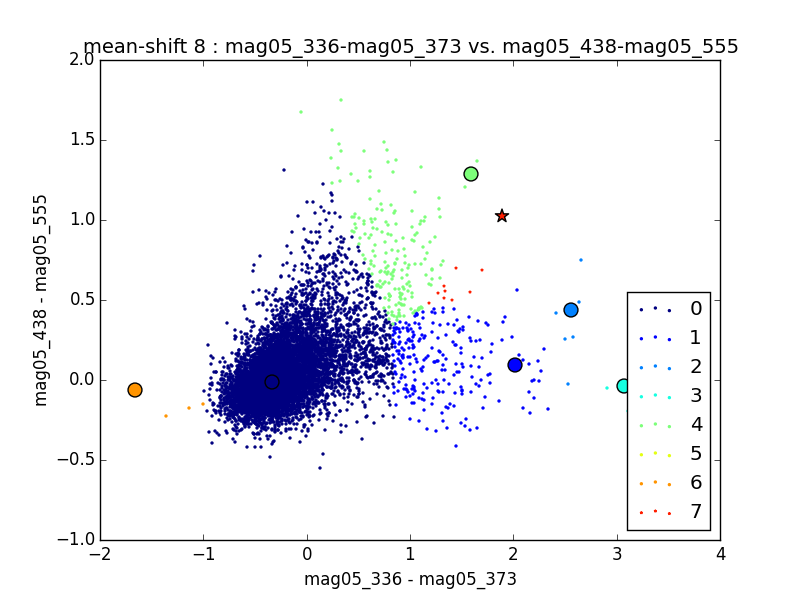
\includegraphics[width=\linewidth]{figs/meanshift_color_8cl_mag05_336-mag05_373vsmag05_438-mag05_555}
\caption{Colour-Colour distribution of the $U-O_{2}$ and B-V colours, clustered using Meanshift with $h=0.33$. The colour of each point corresponds to the cluster the point was assigned to. Cluster numbers can be seen in the legend.}
\label{fig:UOIIMS}
\end{figure}

The K-Means algorithm produced more reliable results, as it produced clusters of relatively similar sizes.
As K increased, the sum of squares value for each clustering decreased, a trend that is expected.
The silhouette score was a maximum at $K=3$, and elbowed at $K=5$. Both clusterings were investigated to determine which was optimal.
At $K=3$, the distribution was segmented according to its U - OII colour.
At $K=5$, the segmentation was similar, however, the section of data that was significantly red in the U-OII colour was given its own cluster.

With each combination of broad bands, the same patterns existed.
This combination in 2-Dimensions did not seem to uncover any more detail or interesting objects than the UVW-U combinations.

\subsubsection{3-Dimensions}

Following the initial clustering, the colours were each broken down into a combination of the OII band and each other band.
The colours used in three dimensions were a combination of U-OII, OII-B, OII-V, and OII-I.

The clustering performance in three dimensions was generally better for almost all clustering parameters.
With all combinations, the clustering algorithms were able to identify a large branch of objects that was fairly red in the U-OII colour, and very blue in the other two, see Figure ~\ref{fig:UOIIKM3d}.
This branch was identified at all values of K, and most values of h.
The added complexity of three dimensions removed the restrictions of only using two dimensions, and allowed the algorithms to cluster the distributions more accurately.

\begin{figure}
\centering
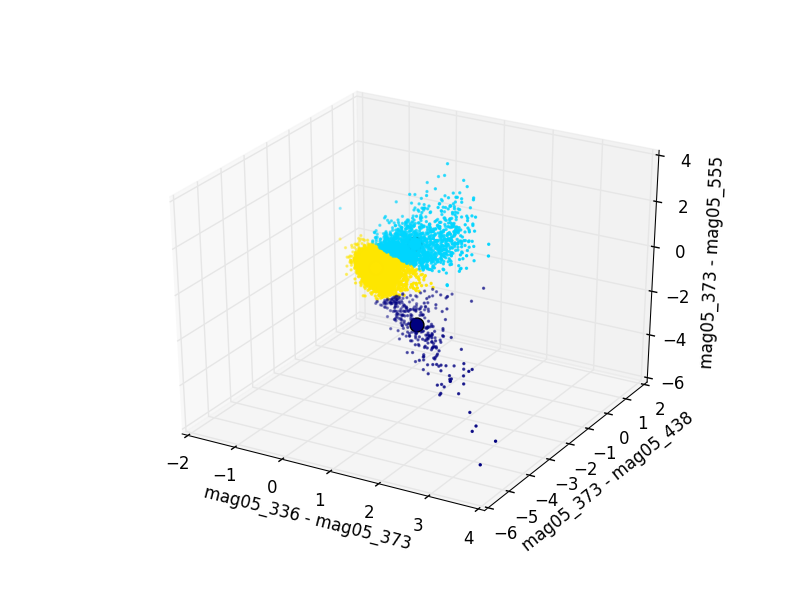
\includegraphics[width=\linewidth]{figs/kmeans_3d_color_3cl_mag05_336-mag05_373vsmag05_373-mag05_438vsmag05_373-mag05_555}
\caption{Colour-Colour distribution of the $U-O_{2}$, $O_{2}-B$, and $O_{2}-V$ colours, clustered using K-Means with $K=3$. The colour of each point corresponds to the cluster the point was assigned to. Cluster numbers can be seen in the legend.}
\label{fig:UOIIKM3d}
\end{figure}

The optimal meanshift clustering was not as apparent in three dimensions.
In the OII - B vs. OII - V combination, the score and number of clusters did not plateau, and the Meanshift clustering was not considered for the optimal clustering.
However, in the OII - B vs. OII - I and OII - V vs. OII - I combinations, the number of clusters elbowed at an h value that maximized the silhouette score.
The number of clusters elbowed at 5, over a range of h values for both combinations.
In each case, the algorithm was able to pick out groups of outliers more clearly than in two dimensions, and the elbow point was taken as the optimal meanshift clustering.

The K-Means algorithm was superior to meanshift for picking out evenly sized groups in all combinations, however, it was not able to pick out some of the detail lying in the groups of outlier data. 
In the combinations that meanshift was successful in, the score peaked at $K=4$, and this was chosen for the optimal clustering. In the last combination, the score peaked at $K=3$.
In addition, each K value was able to pick out the clear branch of objects.
When projected back into two dimensions, the successful segmentation of K-Means can be seen, as it identifies both branches of red objects, and the dense area around zero, see Figure ~\ref{fig:UOIIKM2d}.

\begin{figure}
\centering
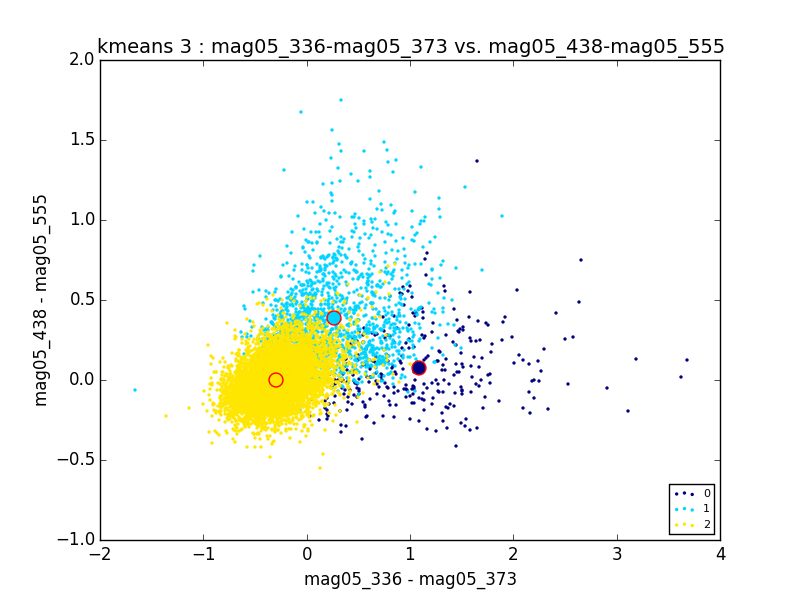
\includegraphics[width=\linewidth]{figs/kmeans_base_color_3cl_mag05_336-mag05_373vsmag05_438-mag05_555}
\caption{Colour-Colour distribution of the $U-O_{2}$ and B-V colours, projected from the 3D clustering using K-Means with $K=3$. The colour of each point corresponds to the cluster the point was assigned to. Cluster numbers can be seen in the legend.}
\label{fig:UOIIKM2d}
\end{figure}

\subsubsection{Astronomy Implications}
Both 2 and 3 dimensional clusterings were investigated in the whitelight image. 
The clusterings in three dimensions were able to segment objects more diffinitively than two dimensions.
This was most noticable in the red branches of the distribution.
In two dimensions, the clusters that segmented the red branches seemed to be a combination of dim point sources and objects in the back of the galaxy or behind clouds.
In three dimensions, these clusters were almost entirely objects in the back of the galaxy or behind clouds instead of the combination.
Additionally, the clusters in three dimensions were better able to detect the boundary between the dense center of the distribution and the outlying branches.
When projected onto the galaxy, the objects dense center of the distribution were located in the densist areas of the spiral arms.
The three dimensional clusterings were able to identify these objects and keep them as a seperate cluster.

\subsection{OIII-V: Unsuccessful Clustering}
The $O_{3}$-V colour was clustered with the U-B colour in two dimensions and the U-$O_{3}$, and B-$O_{3}$ colours in three dimensions.

\subsubsection{2-Dimensions}
The K-Means two dimensional clustering segmented the data into sections of U-B colour.
As K increased, K-Means was able to identify a branch of objects that are bluer in both colours.
The segmentation in the colour-colour space translated into the U-B vs B CMD. 
Each clustering segmented the CMD by U-B colour, and the cluster of bluer objects appears to be a group of objects bright in the U band with a brightest B magnitude of approximately 25.
The K-Means score begins to plateau at K=4, however K=5 has a slightly higher score than the rest of the plateau. This is because K=5 is the first clustering to identify the branch of bluer objects.
Despite the plateau, the clustering scores are not as high as other combinations, and the segmentation appears to be arbitrary. 
The Meanshift clustering does not seem to provide meaningful segmentation. The meanshift parameters do not display the same patterns as other combinations. 
The Meanshift score does not plateau at any number of clusters, and the large center cluster contains almost all of the objects in each segmentation.
Meanshift identifies the branch of blue objects at all bandwidth levels, but as the number of clusters increases the clusters are forced into segmenting the blue objects, not the rest of the distribution.
At $h=0.2$, 8 clusters are produced, and Meanshift identifies many clusters in the blue branch, and a larger cluster of objects that are quite red in the U-B cluster.
This clustering results in a peak in the score.
Despite the identification of different parts of the distribution, the algorithms performance does not match the patterns of other combinations, and seems to be a weak colour combination. 

\subsubsection{3-Dimensions}
The three dimensional distribution displays more structure than two dimensions.
Two clear features are visible, a branch of objects that are red in the U-$O_{3}$ colour, and neutral in the rest, and a second branch of objects that are blue in the $O_{3}$-V colour, red in the B-$O_{3}$ colour, and neutral in the U-$O_{3}$ colour.
At all values of K, K-Means is able to identify the first branch of objects. However, it is not until K=6 that the algorithm is able to identify the second branch as its own cluster, see Figure~\ref{fig:OIIIVKM3d}.
By this point, the algorithm has segmented the dense area of the distribution by its U-$O_{3}$ colour.
When projected into two dimensions, there is significant overlap between the clusters that were segmented by colour, and the first branch of objects does not seem to be its own cluster in two dimensions.
The score at K=6 causes a slight peak in the trend, which signifies the effect of picking out both branches of objects. However, the score is still significantly lower than the clusterings that do not identify these branches.

\begin{figure}
\centering
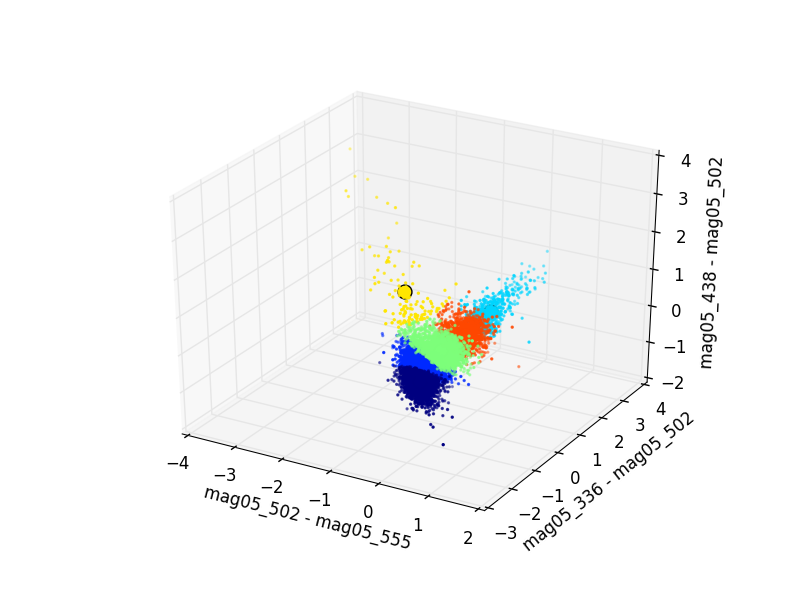
\includegraphics[width=\linewidth]{figs/kmeans_3d_color_6cl_mag05_502-mag05_555vsmag05_336-mag05_502vsmag05_438-mag05_502}
\caption{Colour-Colour-Colour distribution of the U-$O_{3}$, B-$O_{3}$, and $O_{3}$-V colours, clustered using K-Means with $K=6$. The colour of each point corresponds to the cluster the point was assigned to. Cluster numbers can be seen in the legend.}
\label{fig:fig:OIIIVKM3d}
\end{figure}

The Meanshift score plateaued clearly at 7 clusters. There is a large drop in score between 5 and 7 clusters, and both clusterings were able to identify both branches.
Additionally, Meanshift was able to identify sub-clusters within the blue branch of objects, that are objects with extremely blue colours, see Figure ~\ref{fig:OIIIVMS3d}.
The Meanshift clustering was more effective than K-Means, as it did not segment the dense area after it had identified each branch.
The clustering with 5 clusters was chosen as the optimal clustering as the clustering with 7 clusters divided the red branch in two, causing significant overlap in the two and three dimensional spaces.

\begin{figure}
\centering
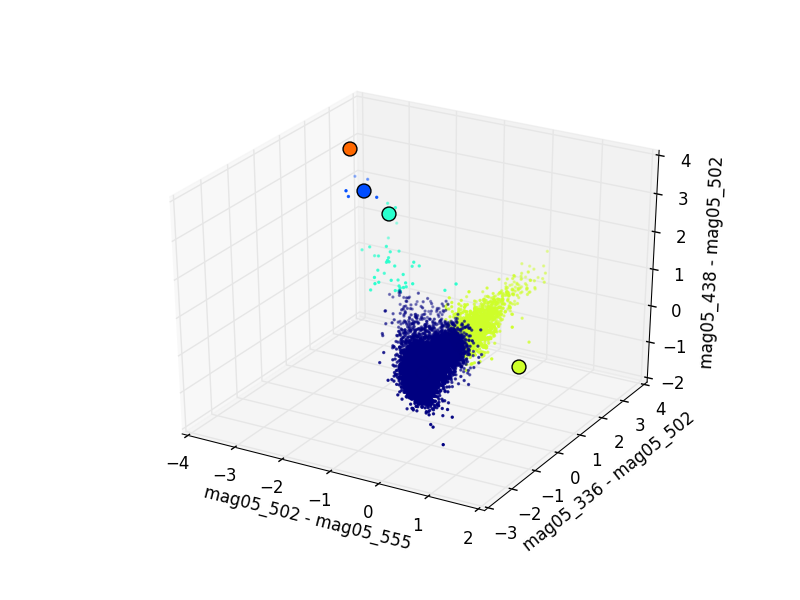
\includegraphics[width=\linewidth]{figs/meanshift_3d_color_5cl_mag05_502-mag05_555vsmag05_336-mag05_502vsmag05_438-mag05_502}
\caption{Colour-Colour-Colour distribution of the U-$O_{3}$, B-$O_{3}$, and $O_{3}$-V colours, clustered using Meanshift with $h=0.5992$. The colour of each point corresponds to the cluster the point was assigned to. Cluster numbers can be seen in the legend.}
\label{fig:fig:OIIIVMS3d}
\end{figure}

\subsubsection{Astronomy Implications}
After investigating each clustering on the whitelight image, most segmentations did not identify sets of objects that were located in specific areas of the galaxy.
Cluster 4 of the strongest Meanshift clustering identified objects that were located in the less dense regions of the spiral arms of M83.
This cluster isolated the branch of red objects in the colour distribution. Additionally, this cluster was clearly defined in the CMD and split the objects at colour 0.
The largest cluster in the blue branch of objects picked isolated objects in the spiral arm, with only one object located in the nucleus.
All of these objects appear to be background galaxy objects or objects behind clouds, as few of the objects appeared in the whitelight image.
The other two clusters that segmented the blue branch were also objects that appear to be background or covered by clouds, indicating that these objects are quite bright in the $O_{3}$ band, and not in the V band.

